\section{Spectral Method}
\begin{comment}
\begin{frame}
	\scriptsize
	Consider
\begin{align}
	\partial_{t}\left(\sin \theta f\right) &+ \textcolor{red}{\partial_\theta\left( \sin ^3 \theta \cos \phi f\right)} - \textcolor{blue}{\partial_x(-\cos\phi \sin\theta \cos\theta f)} \\
	&= \textcolor{red}{D_{r}\left(\partial_\theta \left(\sin \theta \partial_\theta f\right)+ \partial_\phi\left(\frac{1}{\sin \theta} \partial_\phi f\right)\right)}. \nonumber 
\end{align}
	\vspace{12pt}
    \pause
     Ansatz for our \textcolor{cyan}{spectral method}
\begin{align}
	f(\phi, \theta, t) \approx f_0(t) \cdot P_0^0 + \sum_{n=1}^{N} \sum_{i=-2n}^{2n} c^i_{2n}(t) \cdot P^i_{2n}(\phi, \theta), \label{ansatz}
\end{align}
    where $P^i_{2n}(\phi, \theta)$ are harmonic polynomial basis functions. 
\end{frame}
\end{comment}


%%%%%%%%%%%%%%%%%%%%%%%%%
% Von Frau Helzel's Idee
%%%%%%%%%%%%%%%%%%%%%%%%%

\begin{frame}
	Scalar product on $S^2$
	\begin{align*}
		(g,h)_{S^2} := \int_{0}^{2\pi} \int_{0}^{\pi} g(\phi, \theta) h(\phi, \theta) \cdot \sin(\theta) d\theta d\phi
	\end{align*}
	
	\begin{figure}
		\small
		\begin{minipage}{0.46\textwidth}
			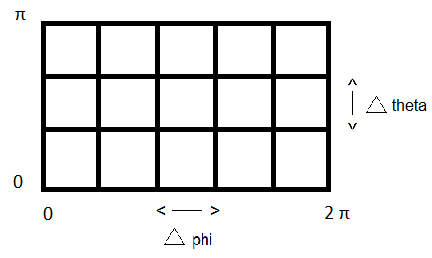
\includegraphics[scale=0.5]{Bilder/Gitter_phi_theta}
		\end{minipage}
		\hfill 
		\begin{minipage}{0.5\textwidth}
			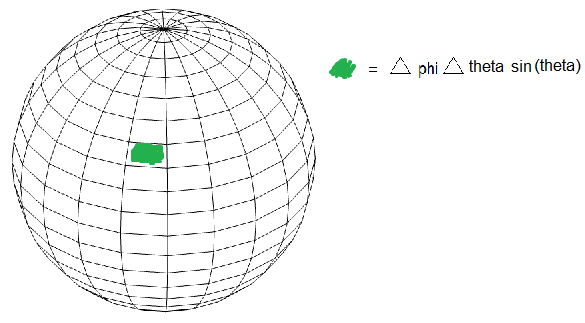
\includegraphics[scale=0.48]{Bilder/Kugel_mit_grid}
		\end{minipage}
		\caption{Grid on sphere}
	\end{figure}
\end{frame}


%%%%%%%%%%%%%%%%%%%%%%
% Properties
%%%%%%%%%%%%%%%%%%%%%%

\begin{frame}{Properties of harmonic polynomial basis functions}
	\begin{itemize}
		\item $\Delta_{S^2}P^i_n = -n(n+1) P^i_n$
		\vspace{12pt}
		\item $	f(\phi, \theta) = f_0 \cdot P_0^0 + \sum_{n=1}^{\infty} \sum_{i=-2n}^{2n} c^i_{2n} \cdot P^i_{2n}(\phi, \theta)$
		\vspace{12pt}
		\item $(P^i_n, P^l_m)_{S^2} = 0, \forall i \neq l \; \text{or} \; n \neq m$
		\vspace{12pt}
		\item $	(P^i_n, P^i_n)_{S^2} = 1$
	\end{itemize}
\end{frame}

\begin{frame}{Harmonic polynomial basis functions}
	\scriptsize
	Basis function ${P}^{i}_{n}(\phi, \theta)$, $n = 0, ..., \infty$ and $i = n, ..., -n$ are computed from orthogonal polynomials (Legendre polynomials). 
	\vspace{20pt}
	\begin{figure}
		\centering
		\subfloat[$P^0_0$]{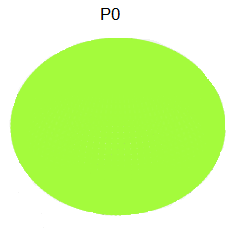
\includegraphics[width=2cm,height=2cm]{Bilder/P0_Kugel}}
		\qquad
		\subfloat[$P^{-1}_2$]{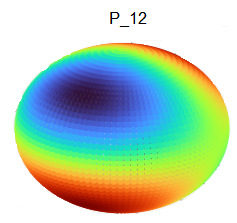
\includegraphics[width=2cm,height=2cm]{Bilder/P_12_Kugel}}
		\qquad
		\subfloat[$P^0_2$]{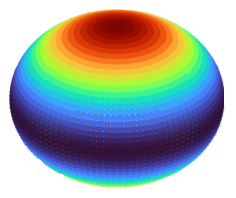
\includegraphics[width=2cm,height=2cm]{Bilder/P02_Kugel}}
		\qquad
		\subfloat[$P^{-1}_4$]{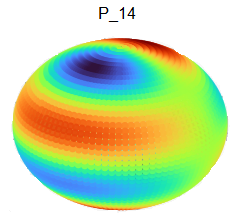
\includegraphics[width=2cm,height=2cm]{Bilder/P_14_Kugel}}
		\caption{Some harmonic polynomial basis functions}
	\end{figure}
	
	\begin{minipage}[b]{0.4\textwidth}
		\begin{table}[H]
			\tiny
			\begin{tabular}{|c|c|}
				\hline
				0th order & 2nd order \\
				\hline
				& $P^{-2}_2 = \sqrt{\frac{15}{16\pi}}\sin^2(\theta)\cos(2\phi)$ \\
				& $P^{-1}_2 = \sqrt{\frac{15}{4\pi}}\sin(\theta)\cos(\theta)\cos(\phi)$ \\
				$P^0_0 = \sqrt{\frac{1}{4\pi}} \cdot 1$ & $P^0_2 = \sqrt{\frac{45}{16\pi}}\cos^2(\theta) - \frac{1}{3}$ \\
				& $P^1_2 = \sqrt{\frac{15}{4\pi}}\sin(\theta)\cos(\theta)\sin(\phi)$\\
				& $P^2_2 = \sqrt{\frac{15}{16\pi}}\sin^2(\theta)\sin(2\phi)$\\
				\hline
			\end{tabular}
		\end{table}
	\end{minipage}
\end{frame}

%%%%%%%%%%%%%%%%%%%%%%%%%%%%%%%%%%%%%%
% Back to the spectral method
%%%%%%%%%%%%%%%%%%%%%%%%%%%%%%%%%%%%%%

\begin{frame}{Spectral method}
	\scriptsize
	Kinetic Smochluchowski equation:
	\begin{align}
		\underbrace{\partial_{t}\left(\sin \theta f\right)}_{[1]} &+ \textcolor{red}{\underbrace{\partial_\theta\left( \sin ^3 \theta \cos \phi f\right)}_{[2]}} - \textcolor{blue}{\underbrace{\partial_x(-\cos\phi \sin\theta \cos\theta f)}_{[3]}} \nonumber \\ 
		&= \textcolor{red}{\underbrace{D_{r}\left(\partial_\theta \left(\sin \theta \partial_\theta f\right)+ \partial_\phi\left(\frac{1}{\sin \theta} \partial_\phi f\right)\right)}_{[4]}}. \label{SmochEq_wx}
	\end{align}	
  Ansatz for our \textcolor{cyan}{spectral method}
 \begin{align}
 	f(\phi, \theta, t) \approx f_0(t) \cdot P_0^0 + \sum_{n=1}^{N} \sum_{i=-2n}^{2n} c^i_{2n}(t) \cdot P^i_{2n}(\phi, \theta), \label{ansatz}
 \end{align}
 where $P^i_{2n}(\phi, \theta)$ are harmonic polynomial basis functions. 
	\vspace{12pt}
	\begin{itemize}
		\item Insert ansatz for $f$ in (\ref{SmochEq_wx}) 
		\item Multiply consecutively with all basis functions used in the ansatz and integrate the resulting equations over $\phi$ and $\theta$
	\end{itemize}
\end{frame}

\begin{frame}{Spectral Method}
	\scriptsize	
	Term [4]: Since $\Delta_{S^2} f = \frac{1}{\sin ^2 \theta} \partial_{\phi \phi} f + \frac{1}{\sin \theta} \partial_\theta\left(\sin \theta \partial_\theta f\right)= -n(n+1) \cdot f$
	
	Term [1]: The time derivative $(c^k_{2n}(t))'$ is obtained as a result.
	
	Term [2]: Inserting the ansatz for $f$ into Term [2], we define:
	\begin{align}
		z_0(\phi, \theta) &= \left[\partial_\theta( \sin ^3 \theta \cos \phi (c^0_0 P^0_0))\right], \\
		z(\phi, \theta) &= \sum_{n = 1}^{N} \, \sum_{k=-2n}^{2n} \left[\partial_\phi (b_\phi (c^k_{2n} P^{k}_{2n})) + \partial_\theta(\sin \theta b_\theta (c^k_{2n} P^{k}_{2n}))\right]. \label{smoch_ansatz}
	\end{align}
\end{frame}


\begin{frame}
\scriptsize
Then do a projection onto all the polynomials $P^{k}_{2n}(\phi, \theta)$ and integrate the result over $S^2$ to determine the coefficients $f_0$ and $c^k_{2n}$

\begin{align*}
	f_0(t) &=  \int_{0}^{2\pi} \int_{0}^{\pi} z_0(\phi, \theta) \cdot P^{k}_{2n}(\phi, \theta) \, \sin\theta d\theta d\phi. \\
	c^k_{2n}(t) &= \int_{0}^{2\pi} \int_{0}^{\pi} z(\phi, \theta) \cdot P^{k}_{2n}(\phi, \theta) \, \sin\theta d\theta d\phi.
\end{align*}

\end{frame}

\begin{frame}{Hierarchy of Moment Equations for Shear Flow 1D}
	\scriptsize
	For  $f(\phi, \theta, t) = c^0_0(t) + \sum_{i=-2}^{2} c^i_{2}(t) \cdot P^i_{2}(\phi, \theta)$,i.e. N=1, we obtain the following system
	\begin{align*}
		\partial_{t} f_0 = &-\textcolor{blue}{\frac{\sqrt{15}}{15}\partial_x c^{-1}_2}\\
		\partial_{t} c^{-2}_2 = &-\textcolor{blue}{\frac{1}{7} \partial_x c^{-1}_2} -\textcolor{red}{6D_rc^{-2}_2}+ \textcolor{red}{\frac{2}{7}w_xc^{-1}_2} \\
		\partial_{t} c^{-1}_2 = &-\textcolor{blue}{\frac{\sqrt{15}}{15}\partial_x f_0} - \textcolor{blue}{\frac{1}{7} \partial_x c^{-2}_2} - \textcolor{blue}{\frac{\sqrt{3}}{21}\partial_x c^0_2} \\ &-\textcolor{red}{\frac{5}{7}w_x c^{-2}_2} -\textcolor{red}{6D_r c^{-1}_2} +\textcolor{red}{\frac{3\sqrt{3}}{7}w_x c^0_2} \\
		\partial_{t} c^0_2 = &-\textcolor{blue}{\frac{\sqrt{3}}{21}\partial_x c^{-1}_2} -\textcolor{red}{\frac{4\sqrt{3}}{7}w_x c^{-1}_2} -\textcolor{red}{6D_r c^0_2} \\
		\partial_{t} c^1_2 = &-\textcolor{blue}{\frac{1}{7}\partial_x c^2_2} -\textcolor{red}{-6Dr c^{1}_2} -\textcolor{red}{\frac{5}{7}w_x c^{2}_2}\\
		\partial_{t} c^2_2 = &-\textcolor{blue}{\frac{1}{7}\partial_x c^1_2} +\textcolor{red}{\frac{2}{7}w_x c^{1}_2} -\textcolor{red}{6D_r c^{2}_2}
	\end{align*}
\end{frame}
\begin{frame}{Example for a One-Dimensional Shear Flow}
	\scriptsize
     We obtain for the \textcolor{red}{Drift Diffusion term} \\
	
	\begin{equation*}
		\partial_t \left(\begin{array}{c}
			f_0 \\
			c_2^{-2} \\
			c_2^{-1} \\
			c_2^0 \\
			c_2^1 \\
			c_2^2
		\end{array}\right)  = \begin{pmatrix}
			0 & 0 & 0 & 0 & 0 & 0 \\
			0 & -6D_r & \frac{2}{7}w_x & 0 & 0 & 0 \\
			-\frac{\sqrt{15}}{5}w_x & -\frac{5}{7}w_x & -6D_r & \frac{3\sqrt{3}}{7}w_x & 0 & 0 \\
			0 & 0 & -\frac{4\sqrt{3}}{7}w_x & -6D_r & 0 & 0 \\
			0 & 0 & 0 & 0 & -6D_r & -\frac{5}{7} w_x\\
			0 & 0 & 0 & 0 & \frac{2}{7}w_x & -6D_r
		\end{pmatrix} \cdot
		\left(\begin{array}{c}
			0 \\
			c^{-2}_2(t) \\
			c_2^{-1}(t) \\
			c_2^0(t) \\
			c_2^1(t) \\
			c_2^2(t)
		\end{array}\right).
	\end{equation*}
\end{frame}

\begin{frame}
	\scriptsize
	And for the \textcolor{blue}{Spatial term} we get
		$$
	\partial_t \left(\begin{array}{c}
		f_0 \\
		c_2^{-2} \\
		c_2^{-1} \\
		c_2^0 \\
		c_2^1 \\
		c_2^2
	\end{array}\right) + \begin{pmatrix}
		0 & 0 & \frac{\sqrt{15}}{15} & 0 & 0 & 0 \\
		0 & 0 & \frac{1}{7} & 0 & 0 & 0 \\
		\frac{\sqrt{15}}{15} & \frac{1}{7} & 0 & \frac{\sqrt{3}}{21} & 0 &  0 \\
		0 & 0 & \frac{\sqrt{3}}{21} & 0 & 0 & 0 \\
		0 & 0 & 0 & 0 & 0 & \frac{1}{7}\\
		0 & 0 & 0 & 0 & \frac{1}{7} & 0
	\end{pmatrix} \partial_x \left(\begin{array}{c}
		f_0 \\
		c_2^{-2} \\
		c_2^{-1} \\
		c_2^0 \\
		c_2^1 \\
		c_2^2
	\end{array}\right) = 0.
	$$
\end{frame}

